\documentclass[12pt, a4paper]{article}%{{{
\usepackage[utf8]{inputenc}
\usepackage[T1]{fontenc}
\usepackage[a4paper,left=2cm,right=2cm,top=2cm,bottom=2cm]{geometry}
\usepackage[frenchb]{babel}
\usepackage{libertine}
\usepackage{float}
\usepackage{hyperref}
\usepackage{amsfonts}
\usepackage{amssymb}
\usepackage[dvipsnames]{xcolor}
\usepackage[pdftex]{graphicx}

\setlength{\parindent}{0cm}
\setlength{\parskip}{1ex plus 0.5ex minus 0.2ex}
\newcommand{\hsp}{\hspace{20pt}}
\newcommand{\HRule}{\rule{\linewidth}{0.5mm}}

\begin{document}

\begin{titlepage}
  \begin{sffamily}
  \begin{center}

    % Upper part of the page. The '~' is needed because \\
    % only works if a paragraph has started.
    
\includegraphics[scale=1]{Images/polytechnique_genie_gauche_fr_rgb.png}~\\[1.5cm]

    \textsc{\LARGE École Polytechnique Montréal}\\[2cm]

    \textsc{\Large INF8405 : Informatique Mobile}\\[1.5cm]

    % Title
    \HRule \\[0.4cm]
    { \huge \bfseries TP2 : Intégration de Maps\\[0.4cm] }

    \HRule \\[2cm]
    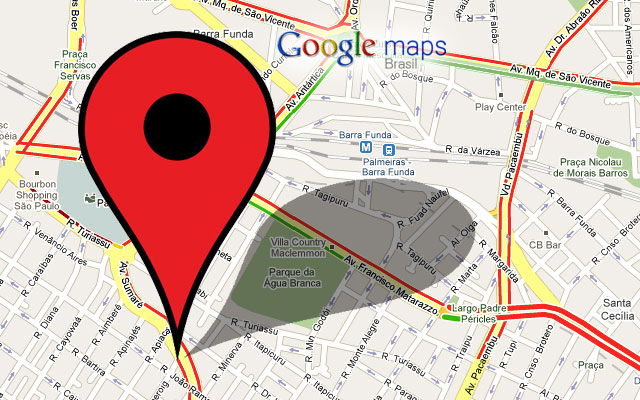
\includegraphics[scale=0.3]{Images/Google-Maps.jpg}\\[2cm]

    % Author and supervisor
    \begin{minipage}{0.4\textwidth}
      \begin{flushleft} \large
          Philippe TROCLET \textsc{1815208}\\
          Alexandre  MAO \textsc{1813566}\\
          Fabien  BERQUEZ \textsc{1800325}\\
      \end{flushleft}
    \end{minipage}
    \begin{minipage}{0.4\textwidth}
      \begin{flushright} \large
        \emph{Soumis à :} M. Aurel Josas RANDOLF\\
        \emph{Soumis le :} 23 Mars 2016  \\
        \emph{Session} Hiver 2016 
      \end{flushright}
    \end{minipage}

    \vfill

  \end{center}
  \end{sffamily}
\end{titlepage}%}}}


\section{Introduction}
\section{Présentation générale}
\section{Présentation Technique}
\section{Critiques et suggestions}
\end{document}
